\title{Controllo di sistemi lineari}
\maketitle
\label{sec:linear-control}

La teoria del controllo dei sistemi lineari è molto robusta e fornisce gli
strumenti... \todo{intro a questo capitolo}

\iffalse
\section{Sistemi lineari}
La definizione di sistema lineare cambia leggermente a seconda di che si parli
di un sistema a tempo continuo o discreto.
È quindi opportuno enunciare la seguente definizione:

\todo{sistema numeraione delle definizioni}
\begin{definition}
    Un \textbf{insieme del tempo} $\mathcal T$ è un sottogruppo di $(\R, +)$.
\end{definition}
Nella pratica, $\mathcal T$ coinciderà sempre con $\R$ o con $\Z$, a seconda
che il sistema sia a tempo continuo o discreto, rispettivamente.
Inoltre, quando è definito un insieme del tempo $\mathcal T$, si assume che tutti gli
intervalli siano ristretti a $\mathcal T$.

\begin{definition}[Sistema]
    La quadrupla $\Sigma = (\mathcal T, \mathcal X, \mathcal U, \phi)$,
    dove:
    \begin{itemize}
        \item $\mathcal T$ è un insieme del tempo.
        %zzz
        \item $\mathcal X$ è un insieme non vuoto, detto \textbf{spazio delle fasi}.
        %
        \item $\mathcal U$ è un insieme non vuoto, detto \textbf{spazio dei controlli ammissibili}.
        %
        \item $\phi: D_\phi \to \mathcal X$ è un'applicazione, detta \textbf{flusso di fase},
        definita su: \\ \\
                $D_\phi :=
                   \left{
                       (\tau, \sigma, x, u) \mid
                       \sigma, \tau \in \mathcal T, \sigma < \tau, x \in \mathcal X, u \in \mathcal U^{[\sigma, \tau)}
                   \right}$, \\ \\
        \todo{non so come avere spacing per questa roba latex kys}
        dove $\mathcal U^{[\sigma, \tau)} := \left{u \mid u: [\sigma, \tau) \to \mathcal U \right}$.
    \end{itemize}
    È detta \textbf{sistema} se valgono le seguenti proprietà:
    \begin{itemize}
        \item \textbf{Non-banalità:}
        \item \textbf{Restrizione:}
        \item \textbf{Semigruppo:}
        \item \textbf{Identità:}
    \end{itemize}
\end{definition}
\fi
%qui sopra devo semplificare un attimo la definizione. Still, do definizione
%di sistema e di sistema lineare.
%la cosa migliore è partire da flusso di fase, dare definizione di campo vettoriale
%e vedere come passare da uuno all'altro.

\section{Sistemi lineari}
\todo{scrivi qualcosa qui}

\subsection{Sistemi dinamici}
Prima di enunciare la definizione di \emph{sistema dinamico}, è necessario che
introduca alcuni concetti.

\begin{definition}
    Un insieme $\mathcal T \subseteq \R^+$ è detto \textbf{insieme del tempo}.
\end{definition}

\begin{definition}
    Un insieme $\Sigma \subseteq \R^{2n}$ è detto \textbf{spazio delle fasi}
    relativo a un sistema fisico quando i vettori
     $\b x \in \Sigma$ rappresentano tutti gli stati possibili
    del sistema, ovvero,
    tutte le $2n$-uple di coordinate e velocità generalizzate $(q_1, \dot q_1, \ldots, q_n, \dot q_n)$
    possibili per il sistema.
\end{definition}
La richiesta che lo spazio delle fasi abbia dimensione pari è dettata dal
fatto che, in generale, per definire lo stato di un sistema meccanico è
necessario conoscere sia il valore delle coordinate generalizzate
che delle rispettive velocità generalizzate associate.
È possibile definire uno spazio delle fasi che abbia dimensione dispari
oppure che sia un insieme dispcreto, ma ciò non è utile per quanto riguarda
questo testo. \todo{magari qui ci sta cit al turchetti che parla di questa roba all'inizio}

\begin{definition}
    Sia $t$ insieme del tempo, $\Sigma$ spazio delle fasi di un sistema e siano $x_0, x(t) \in \Sigma$.
    L'applicazione: \\
    \begin{equation*}
        \begin{array}{cccc}%
            \phi: &\mathcal T \times \Sigma &\to &\Sigma \\
            &\phi^t(x_0) &\mapsto &x(t)
        \end{array}%
    \end{equation*}
    è detta \textbf{flusso di fase} se e solo se rispetta le seguenti proprietà:
    \begin{itemize}
        \item \textbf{Identità:} $\phi^0(x_0) = x_0$.
        \item \textbf{Composizione:} $\phi^t \o \phi^s = \phi^{t+s}$.
        \item \textbf{Conservazione della misura:} esiste una misura $\mu$ di $\Sigma$ %
        conservata $\int_A \det J_\phi \ d\mu = \int_{\phi^t(A)} d\mu$.
    \end{itemize}
\end{definition}

Ora uso le definizioni appena enunciate per introdurre il concetto di
\emph{sistema dinamico}:

\begin{definition}
    La tripla $(\Sigma, \mathcal T, \phi)$ in cui:
    \begin{itemize}
        \item $\Sigma$ è uno spazio delle fasi%
        \item $\mathcal T$ è un insieme del tempo%
        \item $\phi$ è un flusso di fase%
    \end{itemize}
    è detta \textbf{sistema dinamico}.
\end{definition}

A seconda di come è costruito il flusso di fase, un sistema dinamico
può essere categorizzato come \emph{lineare} o\emph{non lineare}.
Inoltre, a seconda della scelta di $\mathcal T$, il sistema è detto
\emph{a tempo continuo} oppure \emph{a tempo discreto}.
L'esempio \ref{ex:semaforo} mostra come è possibile costruire
il più semplice sistema dinamico.

\begin{example}
    \label{ex:semaforo}
    Voglio descrivere il comportamento di un semaforo stradale.
    Il semaforo può essere o verde o rosso e cambia colore a intervalli regolari.
    Posso definire lo spazio delle fasi del sistema come:
    \begin{equation*}
        \Sigma := \{\text{Verde}, \text{Rosso} \}.
    \end{equation*}
    Il tempo è discreto: $\mathcal T = \Z^+$ e definisco il flusso di fase $\phi$:
    \begin{equation*}
        \phi^t(\text Rosso) = \left\{
        \begin{array}{lrl}
            Verde &$t$ &dispari\\
            Rosso &$t$ &pari
        \end{array}
        \right.
    \end{equation*}
    \begin{equation*}
        \phi^t(\text Verde) = \left\{
        \begin{array}{lrl}
            Rosso &$t$ &dispari\\
            Verde &$t$ &pari
        \end{array}
        \right.
        .
    \end{equation*}
    La tripla $(\Sigma, \mathcal T, \phi)$ è un \emph{sistema dinamico}.
    Il sistema è illustrato in figura \ref{fig:esempio-semaforo}.
    \begin{figure}[H]
        \centering
        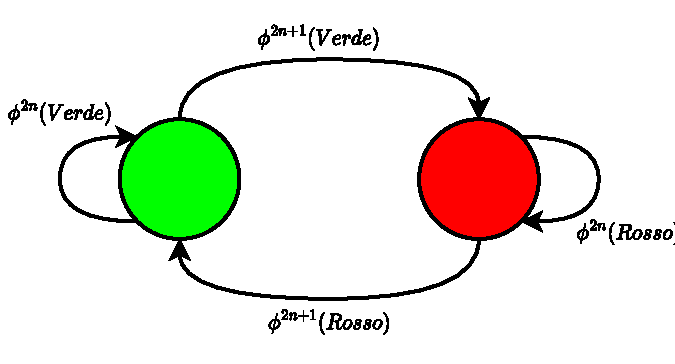
\includegraphics[width=0.5\textwidth]{assets/ex-semaforo}
        \caption[Semaforo]{Esempio di un semaforo come sistema dinamico.
        Gli stati possibili del sistema sono i due colori e il flusso di fase
        regola l'evoluzione temporale del sistema.}
        \label{fig:esempio-semaforo}
    \end{figure}
\end{example}


In generale, dalla osservazione di un sistema fisico si riesce a costruire un campo vettoriale
di equazioni differenziali che ne descrive il moto:
\begin{equation*}
    \dot {\b x} (t) = \b a(\b x).
\end{equation*}
È naturale quindi chiedersi come \emph{e se} sia possibile ricavare il flusso di fase partendo
dal campo vettoriale (e viceversa).
Si può dimostrare \todo{devo mettere la dimostrazione?} che vale la relazione~\eqref{eq:campo-vettoriale},
che mette quindi in relazione ogni sistema di equazioni differenziali con un rispettivo sistema dinamico.
\begin{equation}
    \b a (\b x) = \left.\frac d {dt} \right| _{t=0} \phi^t (\b x_0).
    \label{eq:campo-vettoriale}
\end{equation}

La \eqref{eq:campo-vettoriale} è, in generale, impossibile da integrare analiticamente.
Tuttavia, per i sistemi lineari, esiste una soluzione in forma chiusa al problema.
Questa proprietà dei sistemi lineari è molto utile, visto che permette di trasformare un sistema
da tempo continuo a tempo discreto e viceversa.
Mostrerò come nel paragrafo seguente.
\todo{eventualmente, posso fare un esempio di campo vettoriale mostrando il flow delle fasi...
Non so se serve, per ora non lo faccio.}


\subsection{Equazioni differenziali lineari}
\label{subsec:equazioni-differenziali-lineari}
Iniziamo con due righe di teoria sulle equazioni differenziali:

\begin{definition}
    Sia $\b x = \b x(t) \in \R^n$, $A \in \M_{2\times 2}(\R)$. Un'equazione nella forma
    \begin{equation}
        \dot{\b x} = A \b x
        \label{eq:sistema-lineare}
    \end{equation}
    è detta \textbf{equazione differenziale omogenea (\textsc{ODE}) lineare di \rom{1} ordine.}
    \label{def:sistema-lineare}
\end{definition}
\todo {glossario e small caps}

Per le ODE di questo tipo esiste una soluzione analitica data da
\begin{equation}
    \b x(t) = e^{\b A t} \b x(0).
    \label{eq:soluzione-lineare}
\end{equation}
Basta infatti sostituire la definizione di esponenziale di matrice
\begin{equation}
    e^{A} := \sum_{k=0}^{+\infty} \frac{A^k}{k!}
    \label{eq:exp-matrice}
\end{equation}
nell'equazione \eqref{eq:sistema-lineare} e verificare che si ottiene un'identità.
Inoltre, il \emph{Teorema di Esistenza e Unicità} ci garantisce che questa soluzione
trovata è unica.

\paragraph{}
Ora, prendo in considerazione un sistema dinamico che ha come campo vettoriale associato
l'equazione \eqref{eq:sistema-lineare}. Osservo che la soluzione \eqref{eq:soluzione-lineare}
corrisponde proprio al flusso di fase associato al sistema. Infatti, se prendo
$\phi^t(\b x) = e^{At} \b x$ e lo inserisco nella \eqref{eq:campo-vettoriale},
trovo proprio
\begin{equation*}
    \begin{array}{ll}
        \left. \frac d{dt} \right|_{t=0} e^{At} \b x_0 &= \\
        &= A e^{A0} \b x  \\
        &= A \b x.
    \end{array}
\end{equation*}

\paragraph{}
\todo {aaaa} Qui devo dire qualcosa riguardo alla possibilità di calcolare
esponenziale di matrici per sistemi diagonalizzabili.


\paragraph{}
Questa possibilità di ricavare il flusso di fase partendo dal campo vettoriale per
sistemi lineari vale anche nel caso in cui questi siano \emph{non omogenei}.
Questo fatto ci è molto utile, visto che permetterà di passare da sistemi a tempo
continuo a sistemi a tempo discreto. Vediamo come.

\begin{definition}
    %todo definizione eq non omogenea
    ax +bu
    \label{def:sistema-lineare}
\end{definition}
\todo {glossario e small caps}

%todo
e questa ha soluzione.... Boh


\subsection{Analisi dello spettro di $A$}
In un sistema lineare, le soluzioni asintotiche possono avere tre comportamenti:
0, +inf, oscillare. Questo dipende dagli autovalori...
%todo
e qui mostro nel caso diagonale come funzionano le dinamiche e spiego come l'esponenziale
di matrice sia il mapping che mi fa passare da una cosa all'altra.

\section{Linearizzazione di un sistema}
qua ci metto la teoria delle piccole oscillazioni di bazzani

\section{Controllabilità di un sistema lineare}
Qui devo spiegare che controllabilità equivale a poter spostare gli autovalori a piacimento.
Mostro le condizioni di controllabilità e qualche teoremino. Non so se mettere le
dimostrazioni (no sbatti per ora, magari metto solo le citazioni).

\section{Controllo ottimale: LQR} \todo {glossary LQR}
Qui mi diverto